\documentclass{article}

\usepackage[preprint]{neurips_2024}

\usepackage[utf8]{inputenc}
\usepackage[T1]{fontenc}
\usepackage[hidelinks]{hyperref}
\usepackage{url}
\usepackage{booktabs}
\usepackage{amsfonts}
\usepackage{amsmath}
\usepackage{amssymb}
\usepackage{nicefrac}
\usepackage{microtype}
\usepackage{graphicx}
\usepackage{xcolor}
\usepackage{multirow}
\usepackage{tikz}
\usetikzlibrary{arrows.meta,positioning,shapes.geometric,calc}

\title{When Revision Helps Diffusion LMs, When It Hurts, and Why Honest Compute Matters}
\author{Anonymous Authors}

\begin{document}
\maketitle

\begin{abstract}
Training-free revision methods for diffusion language models are often compared by nominal step counts and justified by uncertainty signals that are never cleanly separated into diagnostic and control roles. We revisit this literature as a compute-normalized diagnostic study rather than a controller paper. Across a focused shortlist of six training-free methods, we show three things. First, honest compute accounting changes key pairwise comparisons and Pareto conclusions on GSM8K: nominal labels hide meaningful differences in actual NFE, latency, throughput, batch size, and compile status. Second, strong diagnostic signals do not reliably become strong controllers under the tested policies: calibration is the strongest observer in our audit, entropy is the most practical signal, and instability does not justify a method-forward win. Third, revision response is task-dependent: the GSM8K story does not transfer cleanly to MATH500, and code results show that shallow syntax repair does not recover execution success. The resulting contribution is a diagnostic study, evaluation protocol, and failure taxonomy for revision in diffusion language models.
\end{abstract}

\section{Introduction}

Training-free inference has become the most active improvement path for diffusion language models (DLMs) as masked diffusion systems such as SEDD, MDLM, LLaDA, and Dream matured into credible open-weight models \citep{lou2024sedd,sahoo2024mdlm,nie2025llada,liu2025dream}. The frontier therefore shifted away from proving that diffusion language modeling is possible and toward deciding how to decode these models efficiently and reliably. That shift produced a growing ecosystem of stopping policies, remasking rules, and fragile-token heuristics \citep{wang2025prophet,li2025saber,zhang2026core}. Yet the literature still tends to conflate three different questions: how much compute a method really uses, whether a signal is a good observer of error, and whether that same signal remains useful once converted into a controller.

This paper argues that these questions should be separated. We do not present another hero controller. Instead, across a focused six-method shortlist and three benchmark roles, we show that a credible study of revision in DLMs must report honest compute, audit observer-controller mismatch, and test whether revision survives a change in task structure. Figure~\ref{fig:teaser} previews the three corresponding takeaways: a compute-order shift on GSM8K, a diagnostic-versus-control gap for the main signals, and a code-boundary failure pattern on HumanEval.

The empirical motivation is straightforward. On GSM8K \citep{cobbe2021gsm8k}, \texttt{CORE-proxy-64} reaches the best raw shortlist accuracy (0.46), but it also runs with \texttt{actual\_nfe}=69, \texttt{latency}=482.95s, \texttt{batch\_size}=1, and \texttt{compile}=false, whereas \texttt{Entropy-Revise-64+3} reaches 0.39 with \texttt{actual\_nfe}=68, \texttt{latency}=210.67s, \texttt{batch\_size}=32, and \texttt{compile}=false. Nominal labels therefore hide a meaningful shift in Pareto interpretation. On the signal side, calibration is the strongest observer in the audit ($d(s)=0.6225$) but offers no deployed control gain, while entropy is useful yet only marginally better than random revision in the lightweight screen. On the task side, GSM8K supports a superficially positive revision story, but MATH500 and HumanEval block a simple generalization: \texttt{Standard-64} leads the MATH500 shortlist at 0.23, and \texttt{Gated TIGER} lowers syntax failure on HumanEval while still trailing \texttt{Standard} on \texttt{pass@1} (0.04 vs.\ 0.06) and worsening runtime failure.

We therefore position the paper as a compute-normalized diagnostic study with three contributions:
\begin{enumerate}
  \item We introduce an honest-compute comparison protocol for training-free DLM revision methods, reporting actual NFE, latency, throughput, batch size, backend, and compile status alongside task metrics.
  \item We show that stronger observation does not reliably become stronger control under the tested interventions, motivating an explicit observer/controller split.
  \item We provide task-dependent boundary evidence across GSM8K, MATH500, and HumanEval, arguing that revision behavior depends on recoverability and structural constraint.
\end{enumerate}

\begin{figure}[t]
\centering
\includegraphics[width=\linewidth]{figures/fig1_teaser.pdf}
\caption{\textbf{Teaser overview.} Left: honest compute changes the GSM8K comparison story. Middle: observer quality and controller gain split apart in the signal audit. Right: syntax repair does not restore execution success at the HumanEval boundary.}
\label{fig:teaser}
\end{figure}

\section{Related Work}

The relevant literature spans three threads. The first is the DLM architecture line itself, from early discrete diffusion systems to scaled masked diffusion models such as SEDD, MDLM, LLaDA, and Dream \citep{lou2024sedd,sahoo2024mdlm,nie2025llada,liu2025dream}. The second is training-free acceleration and selective computation, including stopping, skipping, caching, and parallel unmasking strategies \citep{wang2025prophet,zhang2025fastdllm,zhao2025ebsampler,dai2026surelock}. The third is revision and remasking, where methods revisit positions deemed fragile, uncertain, or unstable after a draft pass \citep{li2025saber,zhang2026core,kim2026starr,lee2026cover}.

Our paper differs from all three lines in emphasis. It does not introduce a new diffusion backbone. It does not present a new acceleration primitive. It does not claim a new best revision controller. Instead, it asks what conclusions remain once these methods are compared under a shared runtime-fairness protocol and once their signals are interpreted separately as observers and controllers.

This framing also changes how calibration enters the story. Prior work often uses confidence or entropy as operational inputs to a policy, while the broader calibration literature treats uncertainty quality as a first-class measurement problem \citep{guo2017calibration,kadavath2022language,xiong2024can}. Here, calibration is primarily a measurement object. Its value is diagnostic: it helps explain why strong uncertainty signals do not automatically translate into strong intervention rules under iterative denoising.

\section{Experimental Protocol}

\subsection{Method Family and Benchmark Roles}

We study six representative methods: \texttt{Standard-64}, \texttt{DNB-84}, \texttt{Prophet-64}, \texttt{CORE-proxy-64}, \texttt{Entropy-Revise-64+3}, and \texttt{TIGER-Instability-64+3}. We deliberately assign different roles to the benchmarks rather than treating them as interchangeable leaderboard rows: GSM8K is the headline reasoning benchmark for honest-compute comparison, MATH500 is the transfer check on a second reasoning regime, and HumanEval is the structural boundary test.

\subsection{Honest-Compute Variables}

For every run we track nominal NFE, actual NFE, latency, throughput, batch size, backend, compile status, and peak VRAM when available. This protocol is necessary because methods with similar names operate under materially different runtime conditions. A comparison that ignores these variables risks overstating both fairness and efficiency.

\subsection{Observer-Controller Split}

We use the language of observers and controllers throughout the paper. An \textbf{observer} is a signal that tracks likely error or revision opportunity. A \textbf{controller} is a policy that acts on that signal. For each signal $s$, we report a diagnostic score $d(s)$ and a control-effectiveness score $g(s)$. Calibration is treated only as an observer in this paper. Entropy-guided and instability-guided revision instantiate controller families.

\begin{figure}[t]
\centering
\resizebox{\linewidth}{!}{%
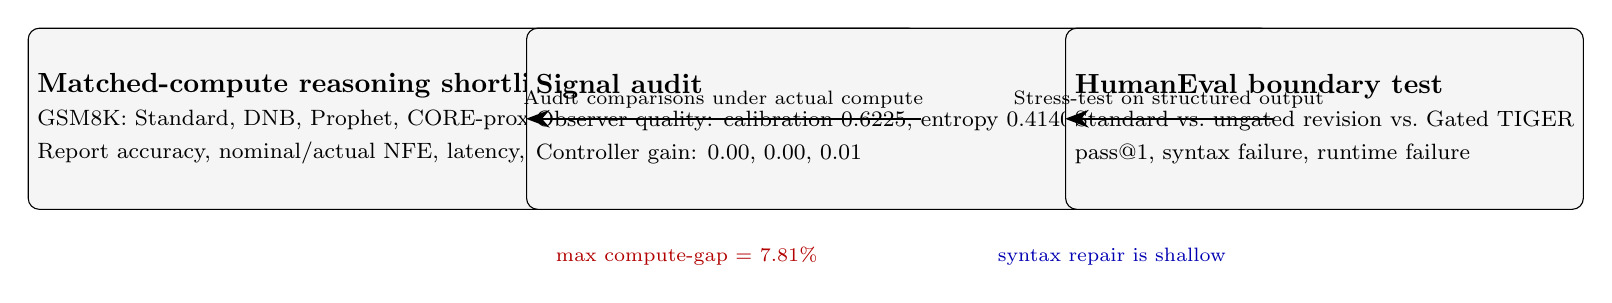
\begin{tikzpicture}[
  x=1cm,y=1cm,
  box/.style={draw, rounded corners=4pt, minimum width=4.15cm, minimum height=2.3cm, align=left, fill=gray!8},
  arrow/.style={-{Stealth[length=3mm]}, thick}
]
\node[box] (a) at (0,0) {\textbf{Matched-compute reasoning shortlist}\\
\footnotesize GSM8K: Standard, DNB, Prophet, CORE-proxy, Entropy, TIGER\\
\footnotesize Report accuracy, nominal/actual NFE, latency, throughput, batch, backend, compile};
\node[box] (b) at (5.4,0) {\textbf{Signal audit}\\
\footnotesize Observer quality: calibration 0.6225, entropy 0.4140, instability 0.0555\\
\footnotesize Controller gain: 0.00, 0.00, 0.01};
\node[box] (c) at (10.8,0) {\textbf{HumanEval boundary test}\\
\footnotesize Standard vs.\ ungated revision vs.\ Gated TIGER\\
\footnotesize pass@1, syntax failure, runtime failure};
\draw[arrow] (a) -- node[above,font=\scriptsize]{Audit comparisons under actual compute} (b);
\draw[arrow] (b) -- node[above,font=\scriptsize]{Stress-test on structured output} (c);
\node[font=\scriptsize, text=red!70!black] at (2.7,-1.75) {max compute-gap = 7.81\%};
\node[font=\scriptsize, text=blue!70!black] at (8.1,-1.75) {syntax repair is shallow};
\end{tikzpicture}
}
\caption{\textbf{Protocol flow.} Our evaluation protocol tracks runtime-fair metadata, audits signal quality separately from control gain, and then tests whether any apparent revision benefit survives a structured-output boundary task.}
\label{fig:protocol}
\end{figure}

\section{Results}

\subsection{Honest Compute Changes Key Comparisons on GSM8K}

Table~\ref{tab:gsm8k} gives the main GSM8K comparison under honest compute.

\begin{table}[t]
\centering
\small
\caption{GSM8K matched-compute shortlist.}
\label{tab:gsm8k}
\resizebox{\linewidth}{!}{%
\begin{tabular}{lcccccccc}
\toprule
Method & Acc. & Nom. NFE & Act. NFE & Latency & Tok/s & Batch & Backend & Compile \\
\midrule
Standard-64 & 0.36 & 64 & 64.00 & 157.04 & 163.01 & 115 & eager & yes \\
DNB-84 & 0.36 & 84 & 83.00 & 180.61 & 141.75 & 115 & eager & yes \\
Prophet-64 & 0.34 & 64 & 63.93 & 147.13 & 173.99 & 57 & eager & yes \\
CORE-proxy-64 & \textbf{0.46} & 64 & 69.00 & 482.95 & 53.01 & 1 & eager & no \\
Entropy-Revise-64+3 & 0.39 & 67 & 68.00 & 210.67 & 121.51 & 32 & eager & no \\
TIGER-Instability-64+3 & 0.39 & 67 & 69.00 & 213.81 & 119.73 & 32 & eager & no \\
\bottomrule
\end{tabular}
}
\end{table}

The main diagnostic point is not that \texttt{CORE-proxy-64} stops being strong. It remains the best raw-accuracy point in the shortlist. The point is narrower and more important: once actual compute is counted, one explicit reorder appears between \texttt{CORE-proxy-64} and \texttt{Entropy-Revise-64+3}, and the Pareto story becomes much less clean than the nominal labels suggest. Figure~\ref{fig:honest_compute} visualizes this result directly by plotting accuracy against latency and annotating actual NFE.

\begin{figure}[t]
\centering
\includegraphics[width=0.92\linewidth]{figures/fig2_honest_compute.pdf}
\caption{\textbf{Pareto view under honest compute.} \texttt{CORE-proxy-64} remains best on raw GSM8K accuracy but has far higher latency than the revision baselines, and the actual-compute ordering differs from the nominal one.}
\label{fig:honest_compute}
\end{figure}

\subsection{Good Observers Do Not Reliably Become Good Controllers}

The signal audit separates diagnostic quality from intervention gain.

\begin{table}[t]
\centering
\small
\caption{Diagnostic-control gap under the tested policies.}
\label{tab:signal_gap}
\begin{tabular}{lccc}
\toprule
Signal & Diagnostic score & Control effectiveness & Gap \\
\midrule
Calibration & 0.6225 & 0.0000 & 0.6225 \\
Entropy & 0.4140 & 0.0000 & 0.4140 \\
Instability & 0.0555 & 0.0100 & 0.0455 \\
\bottomrule
\end{tabular}
\end{table}

Calibration is the clearest example of mismatch: it is the strongest observer and not a useful controller in the current shortlist. Entropy remains diagnostically meaningful, but the lightweight screen shows little gain over random revision. Instability motivates TIGER, yet its observer evidence is weak and its controller does not beat the entropy baseline on GSM8K. Figure~\ref{fig:signal_gap} makes this observer-controller separation visually explicit.

\begin{figure}[t]
\centering
\includegraphics[width=0.82\linewidth]{figures/fig3_signal_gap.pdf}
\caption{\textbf{Observer quality versus controller gain.} The best observer is not the best controller under the tested policies.}
\label{fig:signal_gap}
\end{figure}

\subsection{Revision Response Is Task-Dependent}

The GSM8K story does not transfer cleanly. Table~\ref{tab:task_dep} compares the reasoning shortlist across GSM8K and MATH500.

\begin{table}[t]
\centering
\small
\caption{Ordering across two reasoning datasets.}
\label{tab:task_dep}
\begin{tabular}{lcc}
\toprule
Method & GSM8K & MATH500 \\
\midrule
Standard-64 & 0.36 & \textbf{0.23} \\
CORE-proxy-64 & \textbf{0.46} & 0.21 \\
Entropy-Revise-64+3 & 0.39 & 0.19 \\
TIGER-Instability-64+3 & 0.39 & 0.20 \\
\bottomrule
\end{tabular}
\end{table}

Given the $n=100$ slice, we treat MATH500 as boundary evidence rather than a definitive leaderboard. Even so, it is sufficient to block a simple generalization from ``revision helps on one reasoning benchmark'' to ``revision is a reasoning-wide improvement.''

HumanEval sharpens the structural interpretation. Gating repairs syntax but not executable success.

\begin{table}[t]
\centering
\small
\caption{HumanEval boundary evidence.}
\label{tab:humaneval}
\begin{tabular}{lccc}
\toprule
Method & Pass@1 & Syntax failure & Runtime failure \\
\midrule
Standard & \textbf{0.06} & 0.46 & 0.48 \\
Entropy/TIGER Ungated Revision & 0.02 & 0.48 & 0.50 \\
Gated TIGER & 0.04 & \textbf{0.28} & 0.68 \\
\bottomrule
\end{tabular}
\end{table}

The gate lowers syntax failure by 0.20 relative to ungated revision, but runtime failure worsens by 0.18, and \texttt{pass@1} remains below the standard baseline. Figure~\ref{fig:code_boundary} visualizes that shallow-fix / deep-failure pattern.

\begin{figure}[t]
\centering
\includegraphics[width=0.9\linewidth]{figures/fig4_code_boundary.pdf}
\caption{\textbf{Code boundary failure breakdown.} Syntax improves, but execution success does not recover.}
\label{fig:code_boundary}
\end{figure}

\section{Discussion}

The paper's contribution is strongest when read as a diagnostic study. Honest compute is not a reporting nicety; it is part of the scientific claim. Signals are not interchangeable because their observer and controller roles differ \citep{guo2017calibration,kadavath2022language}. And revision cannot be discussed independently of task structure.

Three cautionary points follow directly from the evidence. First, the honest-compute result should be stated modestly: actual compute changes key comparisons and Pareto conclusions. It does not support a universal ranking rewrite. Second, the observer-controller mismatch should be scoped to the tested policies. Third, the cross-benchmark results remain slice-based ($n=100$ for GSM8K and MATH500 diagnostics, $n=50$ for HumanEval boundary evidence), so the task-dependence story is strong enough to guide framing but not yet strong enough to justify benchmark-standard language.

HumanEval belongs in the paper not as a second success domain but as structural stress-test evidence. That framing matters. The result is more interesting than ``the method failed on code''; it shows that local repair can improve legality without repairing executable semantics when correctness depends on globally constrained structure.

The highest-value next steps are therefore diagnostic rather than algorithmic:
\begin{enumerate}
  \item a benefit-bucket audit separating harmed, fixed, and no-effect cases;
  \item a minimal seed-sensitivity spot-check on the core pairwise comparisons;
  \item appendix-grade runtime fairness and asset-lineage tables.
\end{enumerate}

\section{Conclusion}

We revisited training-free revision in diffusion language models as a diagnostic study rather than a controller paper. Across a focused shortlist, we showed that honest compute changes key comparisons on GSM8K, that strong diagnostic signals do not reliably become strong controllers under the tested policies, and that revision response is task-dependent across reasoning and code.

The resulting recommendation for the field is practical. Future DLM revision papers should report runtime-fairness metadata, separate observer from controller claims, and treat code as a structural stress test rather than as automatic evidence of generality. The current paper does not settle the whole ranking question, but it does provide a more credible protocol for asking it.

\bibliographystyle{plainnat}
\bibliography{references}

\end{document}
